\documentclass{article}
\usepackage[utf8]{inputenc}
\usepackage[english,ngerman]{babel}
%% ========================================================================
%%%% MISC usepackages
%% ========================================================================

%% Chemistry
\usepackage{chemfig,chemmacros}
\chemsetup{modules = all}
\chemsetup[redox]{explicit-sign = true}
\chemsetup[phases]{pos=sub}
%\chemsetup[reactions]{before-tag = {R}, tag-open = [, tag-close = ]}
  
%% Maths
\usepackage{amsmath,amssymb,amsthm,textcomp}

%% Physics
\usepackage{siunitx}

%% Graphics
\usepackage{graphicx}
\usepackage{tikz}
\usepackage{rotating}
%\usepackage{subfig}

%% Tables and Lists
\usepackage{enumerate}
\usepackage{multicol}
\usepackage{geometry}
\usepackage{tabu}
\usepackage{listings}
\usepackage{tabularx}

%% Structures and Style
\usepackage{caption}
\usepackage{subcaption}
\usepackage{booktabs}
\usepackage{colortbl}

\usepackage{xcolor}
\usepackage{xfrac}
\usepackage[export]{adjustbox}[2011/08/13]

\usepackage{booktabs}
\usepackage{float}

\usepackage{fancyhdr}

%% Citing and Settings
\usepackage[backend=biber,
style=numeric,
backref=true, 
natbib=true, %% offering natbib-compatible commands
hyperref=true, %% using hyperref-package references
sorting= none,
doi=true,
maxcitenames=10,
maxbibnames=100,
citestyle=numeric
]{biblatex}

\addbibresource{references.bib}

\usepackage[toc,automake]{glossaries}
\include{abbrevations}
\makeglossaries

\usepackage[colorlinks=true,linkcolor=blue]{hyperref}

%% Figure settings
\renewcommand{\figurename}{Abbildung}
\renewcommand{\tablename}{Tabelle}
\renewcommand{\listfigurename}{Abbildungsverzeichnis}
\renewcommand{\listtablename}{Tabellenverzeichnis}

%% ========================================================================
%%%% Document Information
%% ========================================================================

%% Title
\title{Dünnschicht- und Säulenchromatographie \cite{Versuchsvorschrift}} % Title
\author{Autor: Florian \textsc{Kluibenschedl}} % Author name
\date{Bericht verfasst am: \today} % Date for the report

% Page style - headers
\pagestyle{fancy}
\fancyhf{}
\rhead{PR Allgemeine Chemie A - SS2019}
\lhead{Institut für Allgemeine Chemie - Universität Innsbruck}
\rfoot{Experiment 3 - Seite \thepage}

\begin{document}
  \renewtagform{reaction}[Rgl. ]{}{}
  
  \maketitle % Insert the title, author and date
  
  \begin{center}
    \begin{tabular}{r p{4cm}}
      Versuchsdurchführung am: & 06. März 2019\\ % Date the experiment was performed
      Gruppe, Matrikelnummer: & 3, 11805747 \\
      Lehrveranstaltung: & PR Allgemeine Chemie A \\
      Institut: & Allgemeine, Anorganische und Theoretische Chemie \\
      Assistent: & Wurst Klaus % Instructor/supervisor
    \end{tabular}
  \end{center}


  \begin{abstract}
    Chromatographie ist eine wichtige Disziplin der Chemie und dient zum Trennen von Substanzen einer Mischung. 
    
    Mithilfe von Dünnschichtchromatographie konnte die Zusammensetzung eines Aminosäurengemisches bestimmt werden. Eine Analyse der $R_{f}$-Werte der Probe mit jenen von Referenzsubstanzen zeigte, dass L-Prolin, L-Leucin und L-Arginin enthalten waren. Des weiteren wurde eine Säulenchromatographie zum Trennen von Chlorophyll und Carotin aus einem Blattextrakt von Spinatblättern durchgeführt. Zwei farbige Lösungen wurden erhalten.
  \end{abstract}
  
  \pagebreak
  
  \section{Trennung von Aminosäuren - Dünnschichtchromatographie}
  
    \subsection{Theoretische Grundlagen}
  
      \subsubsection{Motivation} \label{sec:Motivation}
        
        Aminosäuren spielen eine grundlegende Rolle in vielen biochemischen Vorgängen. Werden sie über eine Peptidbindung miteinander verknüpft, bilden sie Polypeptide und in weiterer Folge Proteine. Um nun die oft sehr komplexe Funktionsweise der Proteine besser zu verstehen, ist es notwendig, ihren chemischen Aufbau zu kennen - also die Aminosäurensequenz. Die Möglichkeiten diese zu bestimmen reichen von ausgeklügelten spektroskopischen Methoden über spezifische Abbaureaktionen\footnote{z. B. Hydrolyse der Amidbindung} bis zu chromatographischen Methoden. 
        
        Die Dünnschichtchromatographie ist eine schnelle Methode \cite[S. 148]{TaschenatlasAnallytik}, ein Aminosäurengemisch ohne viel apparativen Aufwand aufzutrennen. Gründe für die Trennung sind Polaritätsunterschiede und verschiedene Dissoziationszustände\footnote{unter den Aminosäuren} bei gleichem \pH-Wert\footnote{Aminosäuren haben typischerweise zwei unterschiedliche \pKa Werte (aufgrund der Carbonsäure- und der Aminogruppe), weswegen bei unterschiedlichen \pH Werten unterschiedliche Ionen zu erwarten sind - das Zwitterion liegt am isoelektrischem Punkt vor}. Durch Vergleich mit Referenzmessungen kann dann die genaue Zusammensetzung vom Aminosäurengemisch bestimmt werden.

      \subsubsection{Ziel des Experiments}
        
        Auf Basis der obigen Überlegungen ist das Ziel, die Zusammensetzung einer Aminosäurenmischung\footnote{mindestens zwei Aminosäuren sind enthalten} zu bestimmen. Die Auswahl ist dabei beschränkt auf L-Serin, L-Leucin, L-Prolin, L-Arginin und L-Histidin.
    
    \subsection{Experimenteller Teil}
  
      \subsubsection{Verwendete Materialien}
              
        \begin{table}[H]
          \centering
          \caption[Materialienliste Dünnschichtchromatographie, Quelle: Autor]{Auflistung der verwendeten Geräte und Chemikalien}
          \label{tab:Materialien}
        
          \begin{tabular}{@{}ll|p{5cm}l@{}}
            \toprule
              Geräte & Hersteller & Chemikalie & Bezogen von \\ \midrule
              2 DC-Platten &  & neutrales Laufmittel - \SI[mode=text]{30}{\milli\litre} \ch{CH3CN}, \SI[mode=text]{20}{\milli\litre} \SI[mode=text]{0.1}{M} \ch{NH4Ac\aq}, \SI[mode=text]{25}{\milli\litre} Ethanol & Vorrat \\
              \SI[mode=text,separate-uncertainty=true]{250}{\milli\litre} Becherglas & DURAN & saures Laufmittel - \SI[mode=text]{30}{\milli\litre} n-Butanol, \SI[mode=text]{10}{\milli\litre} deion. Wasser, \SI[mode=text]{10}{\milli\litre} Eisessig & Vorrat \\
              Uhrglas &  & L-Serin Lösung & Vorrat \\
              Föhn &  & L-Leucin Lösung & Vorrat \\
              Glaskapillaren &  & L-Prolin Lösung & Vorrat \\
              Trockenschrank &  & L-Arginin Lösung & Vorrat \\
              \SI[mode=text]{14}{\centi\meter} Geodreieck und Bleistift & ARISTO & L-Histidin Lösung & Vorrat \\
              Pinzette  &  & \SI[mode=text]{0.1}{\percent} (w/w) Ninhydrin Lösung in Ethanol &  \\
                &  & Probelösung & Vorrat \\ \bottomrule
          \end{tabular}
        \end{table}
        
        Anmerkung zur Handhabung von Ninhydrin\footnote{H und P Sätze: H - 302, 315, 319, 335; P - 261, 305, 351, 338}: Haut, Atemwege und Augen werden gereizt - bei Kontakt mit Wasser spülen
        
      \subsubsection{Versuchsdurchführung} \label{sec:Versuch}
        
        \begin{figure}[H]
          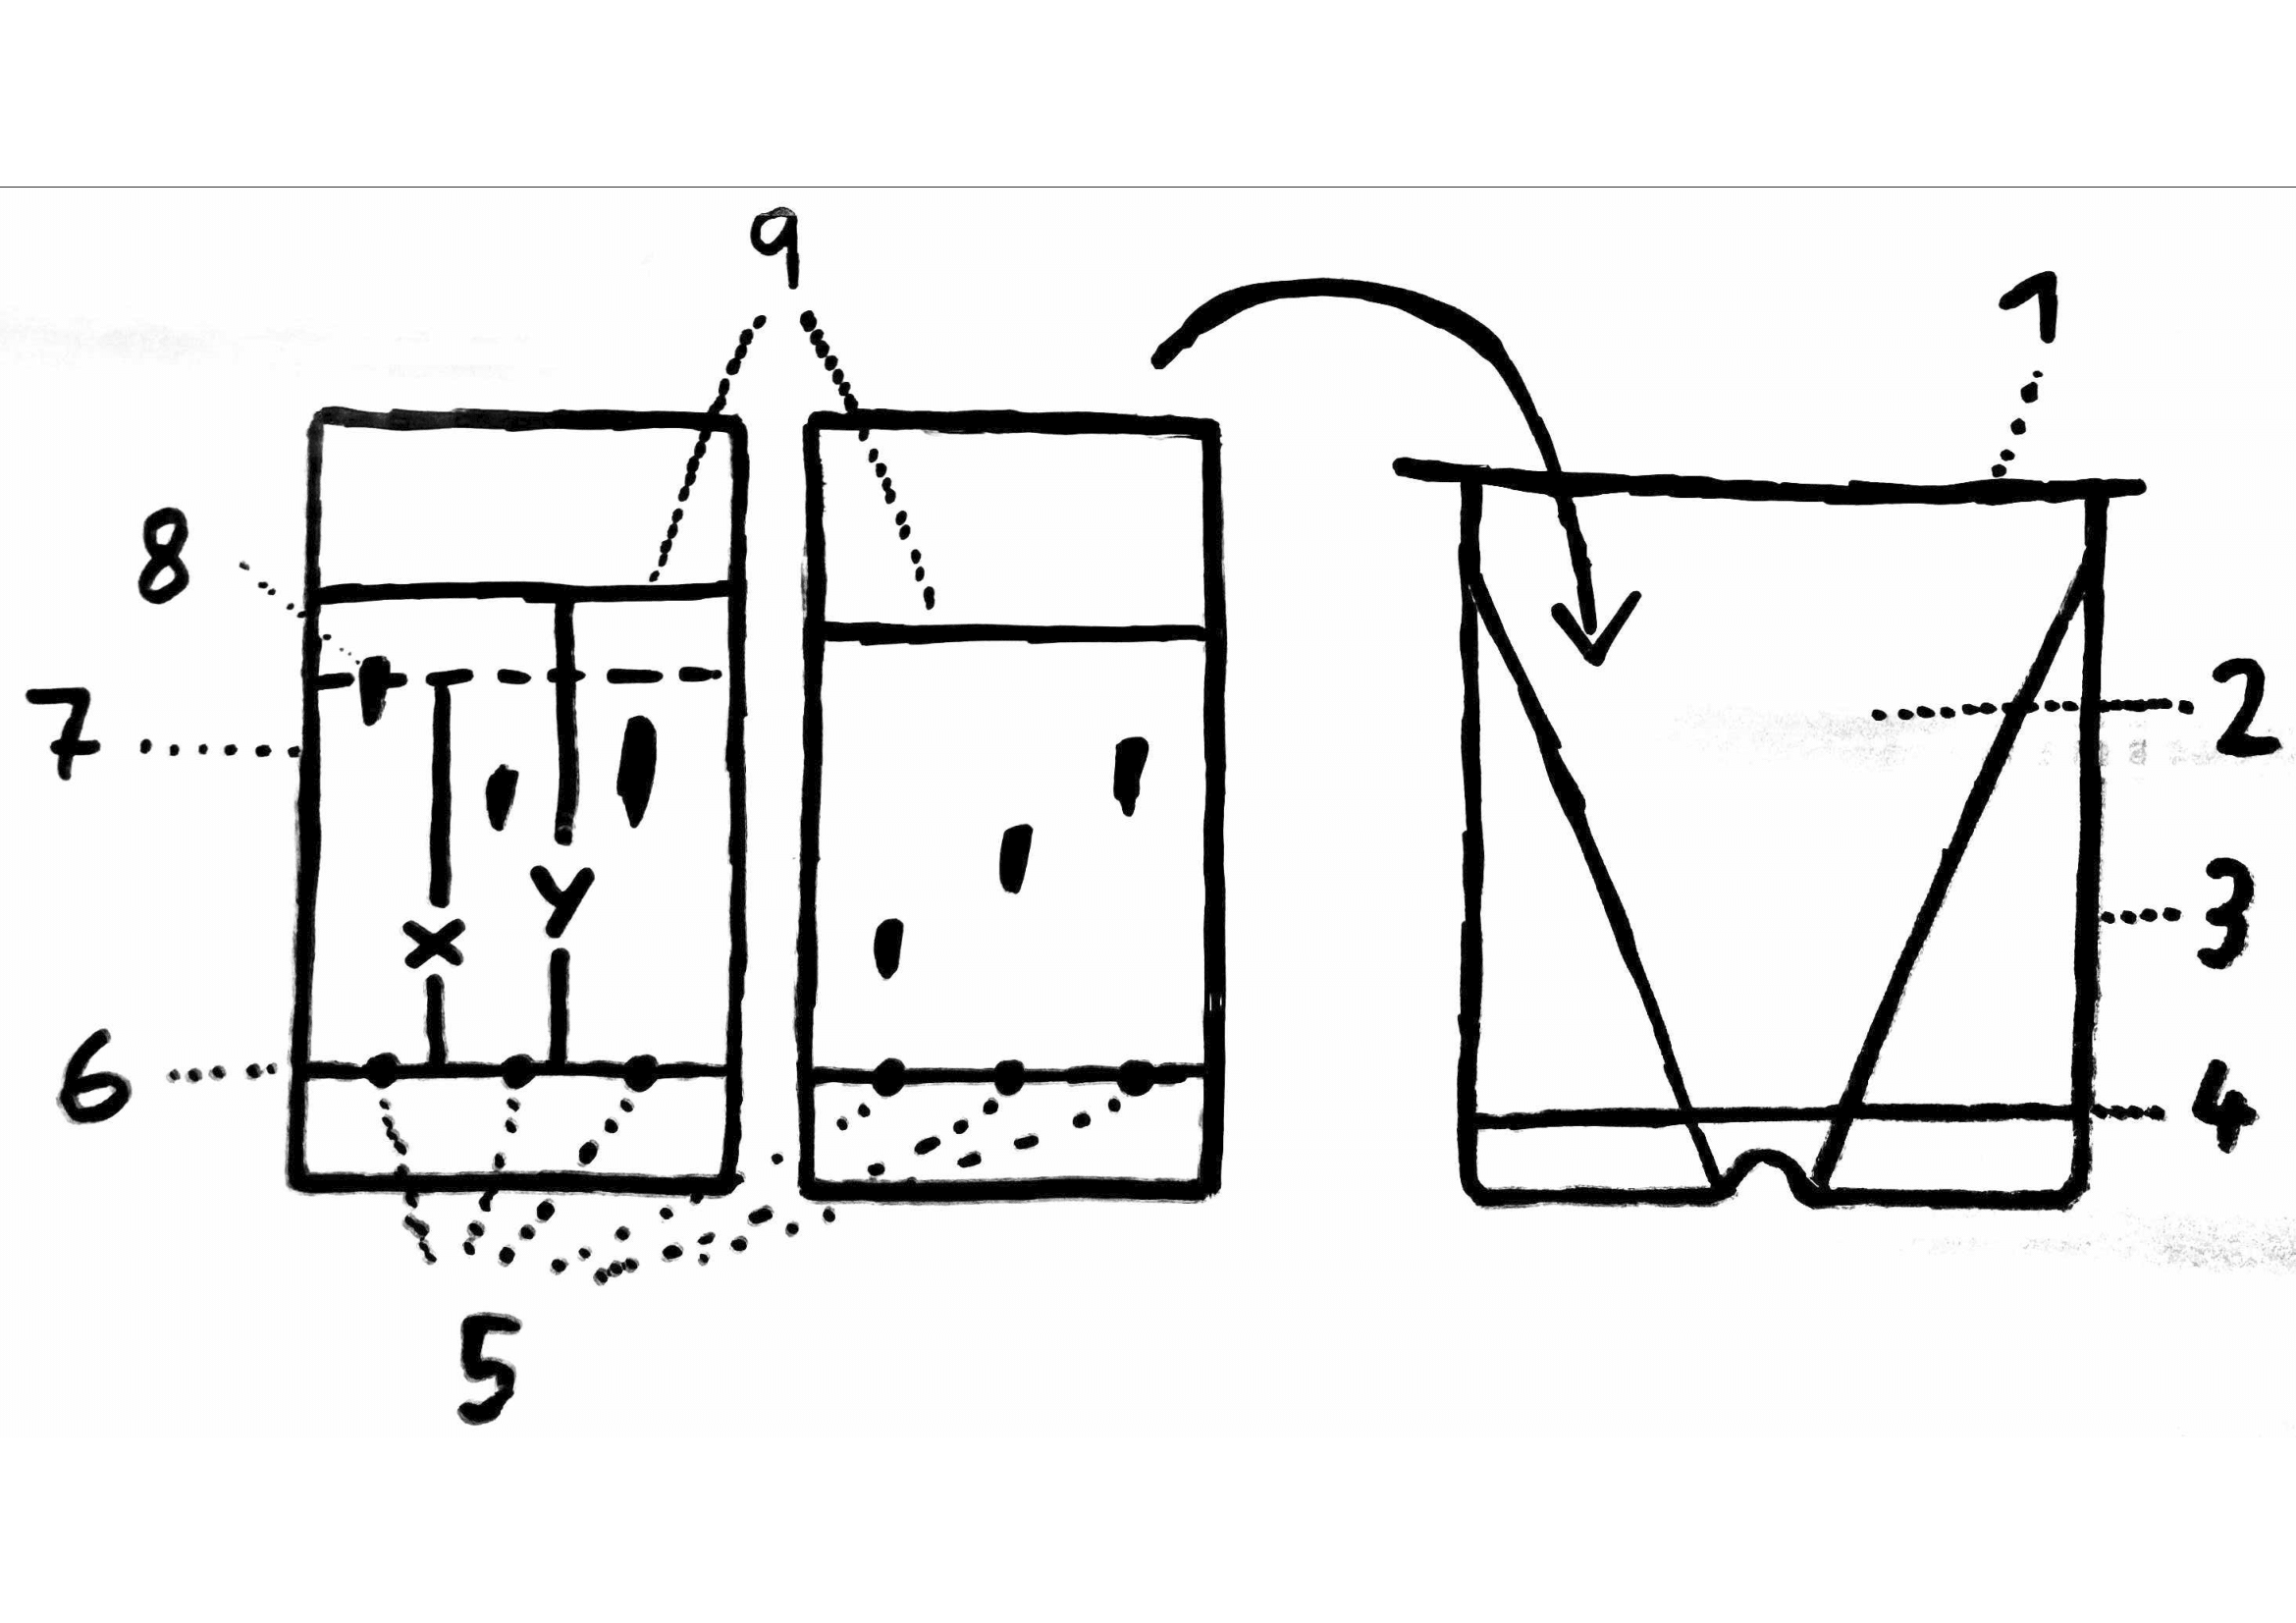
\includegraphics[scale=0.13, center]{Graphiken/Versuchsanordnungen/VersuchsanordnungDC.png} 
          \caption[schematische Versuchsanordnung Dünnschichtchromatographie, Quelle: Autor]{schematische Versuchsanordnung: (1) Uhrglas, (2) mit Lösungsmitteldämpfen gesättigter Gasraum, (3) DC-Kammer - \SI[mode=text,separate-uncertainty=true]{250}{\milli\litre} Becherglas, (4) Laufmittelstand - ca. \SI[mode=text]{0.5}{\centi\meter} über dem Boden des Becherglases, (5) Probespots, (6) mit Bleistift markierte Startlinie, (7) DC-Platte, (8) Probespots nach erfolgter Trennung, (9) Laufmittelfronten - nach Entnahme der DC-Platte mit Bleistift markiert}
          \label{fig:Versuchsanordnung}
        \end{figure}
    
        Zu Beginn wurde die DC-Kammer mit dem jeweiligem Laufmittel\footnote{die Zusammensetzungen sind in Tabelle \ref{tab:Materialien} beschrieben} gefüllt, wie in Abbildung \ref{fig:Versuchsanordnung} beschrieben. Das Becherglas wurde mit einem Uhrglas bedeckt, um das Verdampfen des Lösungsmittels zu verhindern und die DC-Kammer mit dem Lösungsmitteldampf zu sättigen. 
        
        Auf zwei DC-Platten wurde in einer Höhe von \SI[mode=text]{1}{\centi\meter} je eine Startlinie eingezeichnet. Auf dieser wurden dann mithilfe einer Kapillare in regelmäßigem Abstand Probespots der gegebenen fünf Aminosäuren und der zu untersuchenden Probe aufgetragen. Der Probespot wurde dabei zwischen den Spots der Aminosäuren L-Prolin und L-Arginin aufgetragen, da vorherige Praktikumsteilnehmer bei dieser Anordnung die besten Ergebnisse erzielten. Es wurde darauf geachtet, große Probespots zu vermeiden (max. Durchmesser von \SI[mode=text]{2}{\milli\meter}). Nach dem Trocknen der Spots mit einem Föhn wurden die DC-Platten in die wie oben beschrieben präparierten DC-Kammern gestellt und diese mit einem Uhrglas abgedeckt. Die Wanderungsgeschwindigkeit des neutralen Laufmittels war wesentlich schneller wie jene des sauren Laufmittels. Nachdem die Laufmittelfront des neutralen Laufmittels ca. 2/3 der Platte erreichte, wurde sie aus der DC-Kammer entnommen und die Laufmittelfront mit einem Bleistift markiert. Nach dem Trocknen mit einem Föhn wurde die DC-Platte im Abzug mit einer Ninhydrin Lösung besprüht und kurz geföhnt. Anschließend wurde sie im Trockenschrank bei ca. \SI[mode=text]{110}{\degreeCelsius} entwickelt. Nachdem die Laufmittelfront des sauren Laufmittels in etwa die Hälfte der Platte erreichte, wurde sie entnommen und die Laufmittelfront markiert. Nach dem Trocknen und Besprühen mit der Ninhydrin Lösung wurde die Platte ebenfalls im Trockenschrank entwickelt.
    
      \subsubsection{Auswertung}
    
        Aufgrund der in \ref{sec:Motivation} genannten, unterschiedlichen Eigenschaften der untersuchten Proben, halten sich die einzelnen Substanzen verschieden lange in der stationären\footnote{Kieselgel der DC-Platte} bzw. der mobilen \footnote{Laufmittel} Phase auf. Damit legen sie unterschiedliche Strecken auf der DC-Platte zurück, die für eine Substanz bei gleicher Laufmittelzusammensetzung charakteristisch und reproduzierbar sind. Aus der zurückgelegten Strecke der Substanz ($= x$) und der zurückgelegten Strecke des Laufmittels ($= y$) errechnet sich der Retentionsfaktor wie in \eqref{eq:Rf} dargestellt.
    
        \begin{equation}
          R_{f} = \frac{x}{y} \label{eq:Rf}
        \end{equation}
        
        Dieser Wert eignet sich, durch Vergleich mit Referenzen, qualititative Voraussagen über die Zusammensetzung einer Probe zu machen.
        
      \subsubsection{Messergebnisse}
    
        In Tabelle \ref{tab:Messdaten} sind alle Messwerte, die im Rahmen der Versuchsdurchführung wie in \ref{sec:Versuch} beschrieben, gemessen wurden. Zusätzliche Werte für die Auswertung: $y_{sauer}=\SI[mode=text]{3.4}{\centi\meter}$, $y_{neutral}=\SI[mode=text]{4.8}{\centi\meter}$.
      
        \begin{table}[H]
          \centering
          \caption[Messdaten der Dünnschichtchromatographie und daraus abgeleitete Größen, Quelle: Autor]{Messdaten und daraus abgeleitete Größen}
          \label{tab:Messdaten}
            \begin{tabular}{@{}l|ll|ll@{}}
              \toprule
               Substanz & $x_{sauer}$ in \si{\centi\meter} & $R_{f,sauer}$ & $x_{neutral}$ in \si{\centi\meter} & $R_{f,neutral}$ \\ \midrule
               L-Serin & 1.3 & 0.38 & 3.0 & 0.63 \\
               L-Leucin & 2.2 & 0.65 & 3.4 & 0.71 \\
               L-Prolin & 1.0 & 0.29 & 2.5 & 0.52 \\
               L-Arginin & 0.8 & 0.24 & 1.3 & 0.27 \\
               L-Histidin & 0.9 & 0.26 & 1.6 & 0.33 \\ \midrule
               Probe: & 0.8 & 0.24 & 1.3 & 0.27 \\
                      & 1.0 & 0.29 & 2.5 & 0.52 \\
                      & 2.2 & 0.65 & 3.4 & 0.71 \\ \bottomrule
            \end{tabular}
         \end{table}      
      
    \subsection{Ergebnisse und Diskussion}
    
      Die entwickelten DC-Platten zeigen, dass sauber gearbeitet wurde. Die $R_{f}$ Werte konnten bei den meisten Spots gut abgelesen werden, da der Ort der Hauptintensität gut abschätzbar war - siehe Abbildung \ref{fig:DCPlatten}. Lediglich die Bestimmung des $R_{f}$ Wertes bei L-Arginin und L-Histidin war etwas schwieriger, da die beiden Spots in die Länge gezogen waren und einen Schweif bildeten. Dennoch konnte der Ort der vermeintlichen Hauptintensität lokalisiert werden. \\
      
      Ein Vergleich der Spots der Probelösung mit denen der Referenzsubstanzen zeigt, dass 4 der 5 Aminosäuren in der Probe vorhanden sein könnten: L-Prolin, L-Leucin, L-Arginin und L-Histidin. Da die $R_{f}$ Werte von L-Arginin und L-Histidin sehr nahe beieinanderliegen, kann nur durch Vergleich des zugehörigen Spots der Probe mit diesen beiden nicht sicher behauptet werden, ob beide oder doch nur eine vorhanden ist. Die geringe Intensität der Bande des Probespots bei beiden Laufmitteln erschwert die Zuordnung zusätzlich. 
      
      Da der Spot der L-Histidin Lösung auf der mit saurem Laufmittel entwickelten DC-Platte mit der Ninhydrin Lösung eine andere Farbe wie jener der Probe aufweist, kann L-Histidin ausgeschlossen werden. Der Spot von L-Arginin besitzt jedoch diesselbe Farbe wie der Probespot, was die Anwesenheit von L-Arginin bestätigt. Die Probelösung besteht demnach aus einer Mischung von L-Prolin, L-Leucin und L-Arginin.
      
      \begin{figure}[H]
        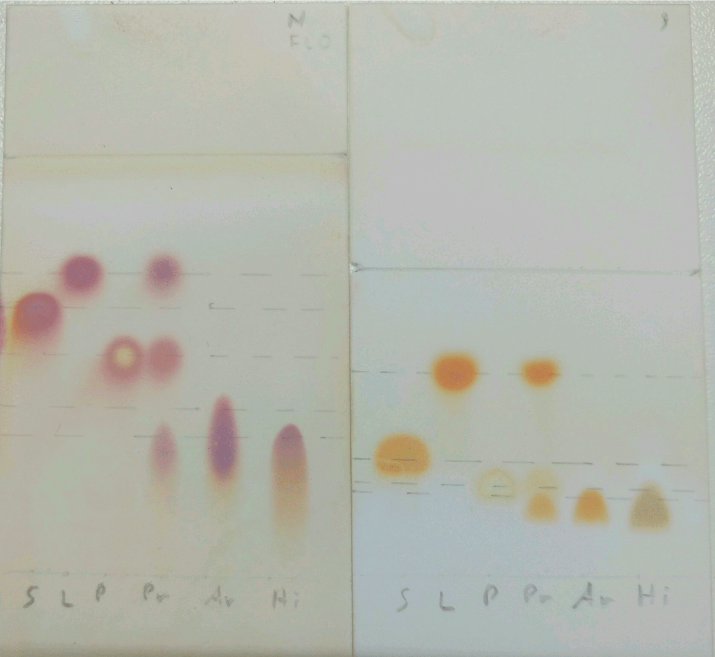
\includegraphics[scale=0.4, center]{Graphiken/Versuchsanordnungen/AusgewerteteDCPlatten.png} 
        \caption[Entwickelte DC-Platten inkl. Beschriftung, Quelle: Autor]{Entwickelte DC-Platten: (links) DC-Platte im neutralen Laufmittel entwickelt, (rechts) DC-Platte im sauren Laufmittel entwickelt - die Spots wurden in folgender Reihenfolge aufgetragen (links nach rechts): L-Serin, L-Leucin, L-Prolin, Probe, L-Arginin, L-Histidin}
        \label{fig:DCPlatten}
      \end{figure}
        
  \pagebreak
  
  \section{Trennung von Pflanzenfarbstoffen - Säulenchromatographie}
  
    \subsection{Theoretische Grundlagen}
    
      \subsubsection{Motivation} \label{sec:Motivationzwei}
      
        Säulenchromatographie ist analog zur Dünnschichtchromatographie eine Methode zum Trennen einer Substanzmischung. Die stationäre Phase ist diesmal in einer Säule gepackt. Die Probe wird am Anfang der Säule aufgegeben und anschließend wird kontinuierlich Eluent (= mobile Phase) hinzugeben. Die Retentionszeit gibt an, wie lang eine Substanz braucht, um durch die Säule zu wandern. Aufgrund der unterschiedlich starken Wechselwirkungen der einzelnen Substanzen mit der stationären Phase, werden die Substanzen getrennt. Der apparative Aufwand ist im Vergleich zur Dünnschichtchromatographie etwas größer, hält sich jedoch in Grenzen \cite[S. 154]{TaschenatlasAnallytik}.\\
        
        Die beiden Biomoleküle Chlorophyll und Carotin nehmen eine bedeutende Rolle im Leben ein. Chlorophyll ist für die grüne Blattfarbe verantwortlich und überlagert zunächst das Carotin. Dieses kommt jedoch zum Vorschein, wenn im Herbst das Chlorophyll systematisch abgebaut wird \cite{DegradationChlorophyll}. 
      
      \subsubsection{Ziel des Experiments}
      
        Um die Eigenschaften der beiden in \ref{sec:Motivationzwei} genannten Moleküle genauer bestimmen zu können, müssen diese zuerst voneinander getrennt werden. Das Ziel des Experiments ist somit, mithilfe von Säulenchromatographie eine entsprechende Trennung durchzuführen. Als Probenmaterial wurden Spinatblätter verwendet.
    
    \subsection{Experimenteller Teil}
    
      \subsubsection{Verwendete Materialien}
        
        \begin{table}[H]
          \centering
          \caption[Materialienliste Säulenchromatographie, Quelle: Autor]{Auflistung der verwendeten Geräte und Chemikalien}
          \label{tab:Materialienzwei}
        
          \begin{tabular}{@{}ll|ll@{}}
            \toprule
              Geräte & Hersteller & Chemikalie & Bezogen von \\ \midrule
              3 Pasteurpipetten mit Saugaufatz &  & Spinatblätter (\textit{lat. Spinacia oleracea}) & Vorrat \\
              \SI[mode=text,separate-uncertainty=true]{50}{\milli\litre} Becherglas & DURAN & Petrolether & Vorrat \\
              Reagenzgläser &  & Ethanol & Vorrat \\
              2 Zentrifugenröhrchen & DURAN & Aceton & Vorrat \\
              Stativ &  & \ch{Al2O3} & Vorrat \\
              Klemmen &  & Watte & Vorrat \\
              \SI[mode=text,separate-uncertainty=true]{10}{\milli\litre} Messzylinder & DURAN & Sand & Vorrat \\ \bottomrule
          \end{tabular}
        \end{table}
        
      \subsubsection{Versuchsdurchführung} \label{sec:Versuchsdurchzwei}
        
        \begin{figure}[H]
          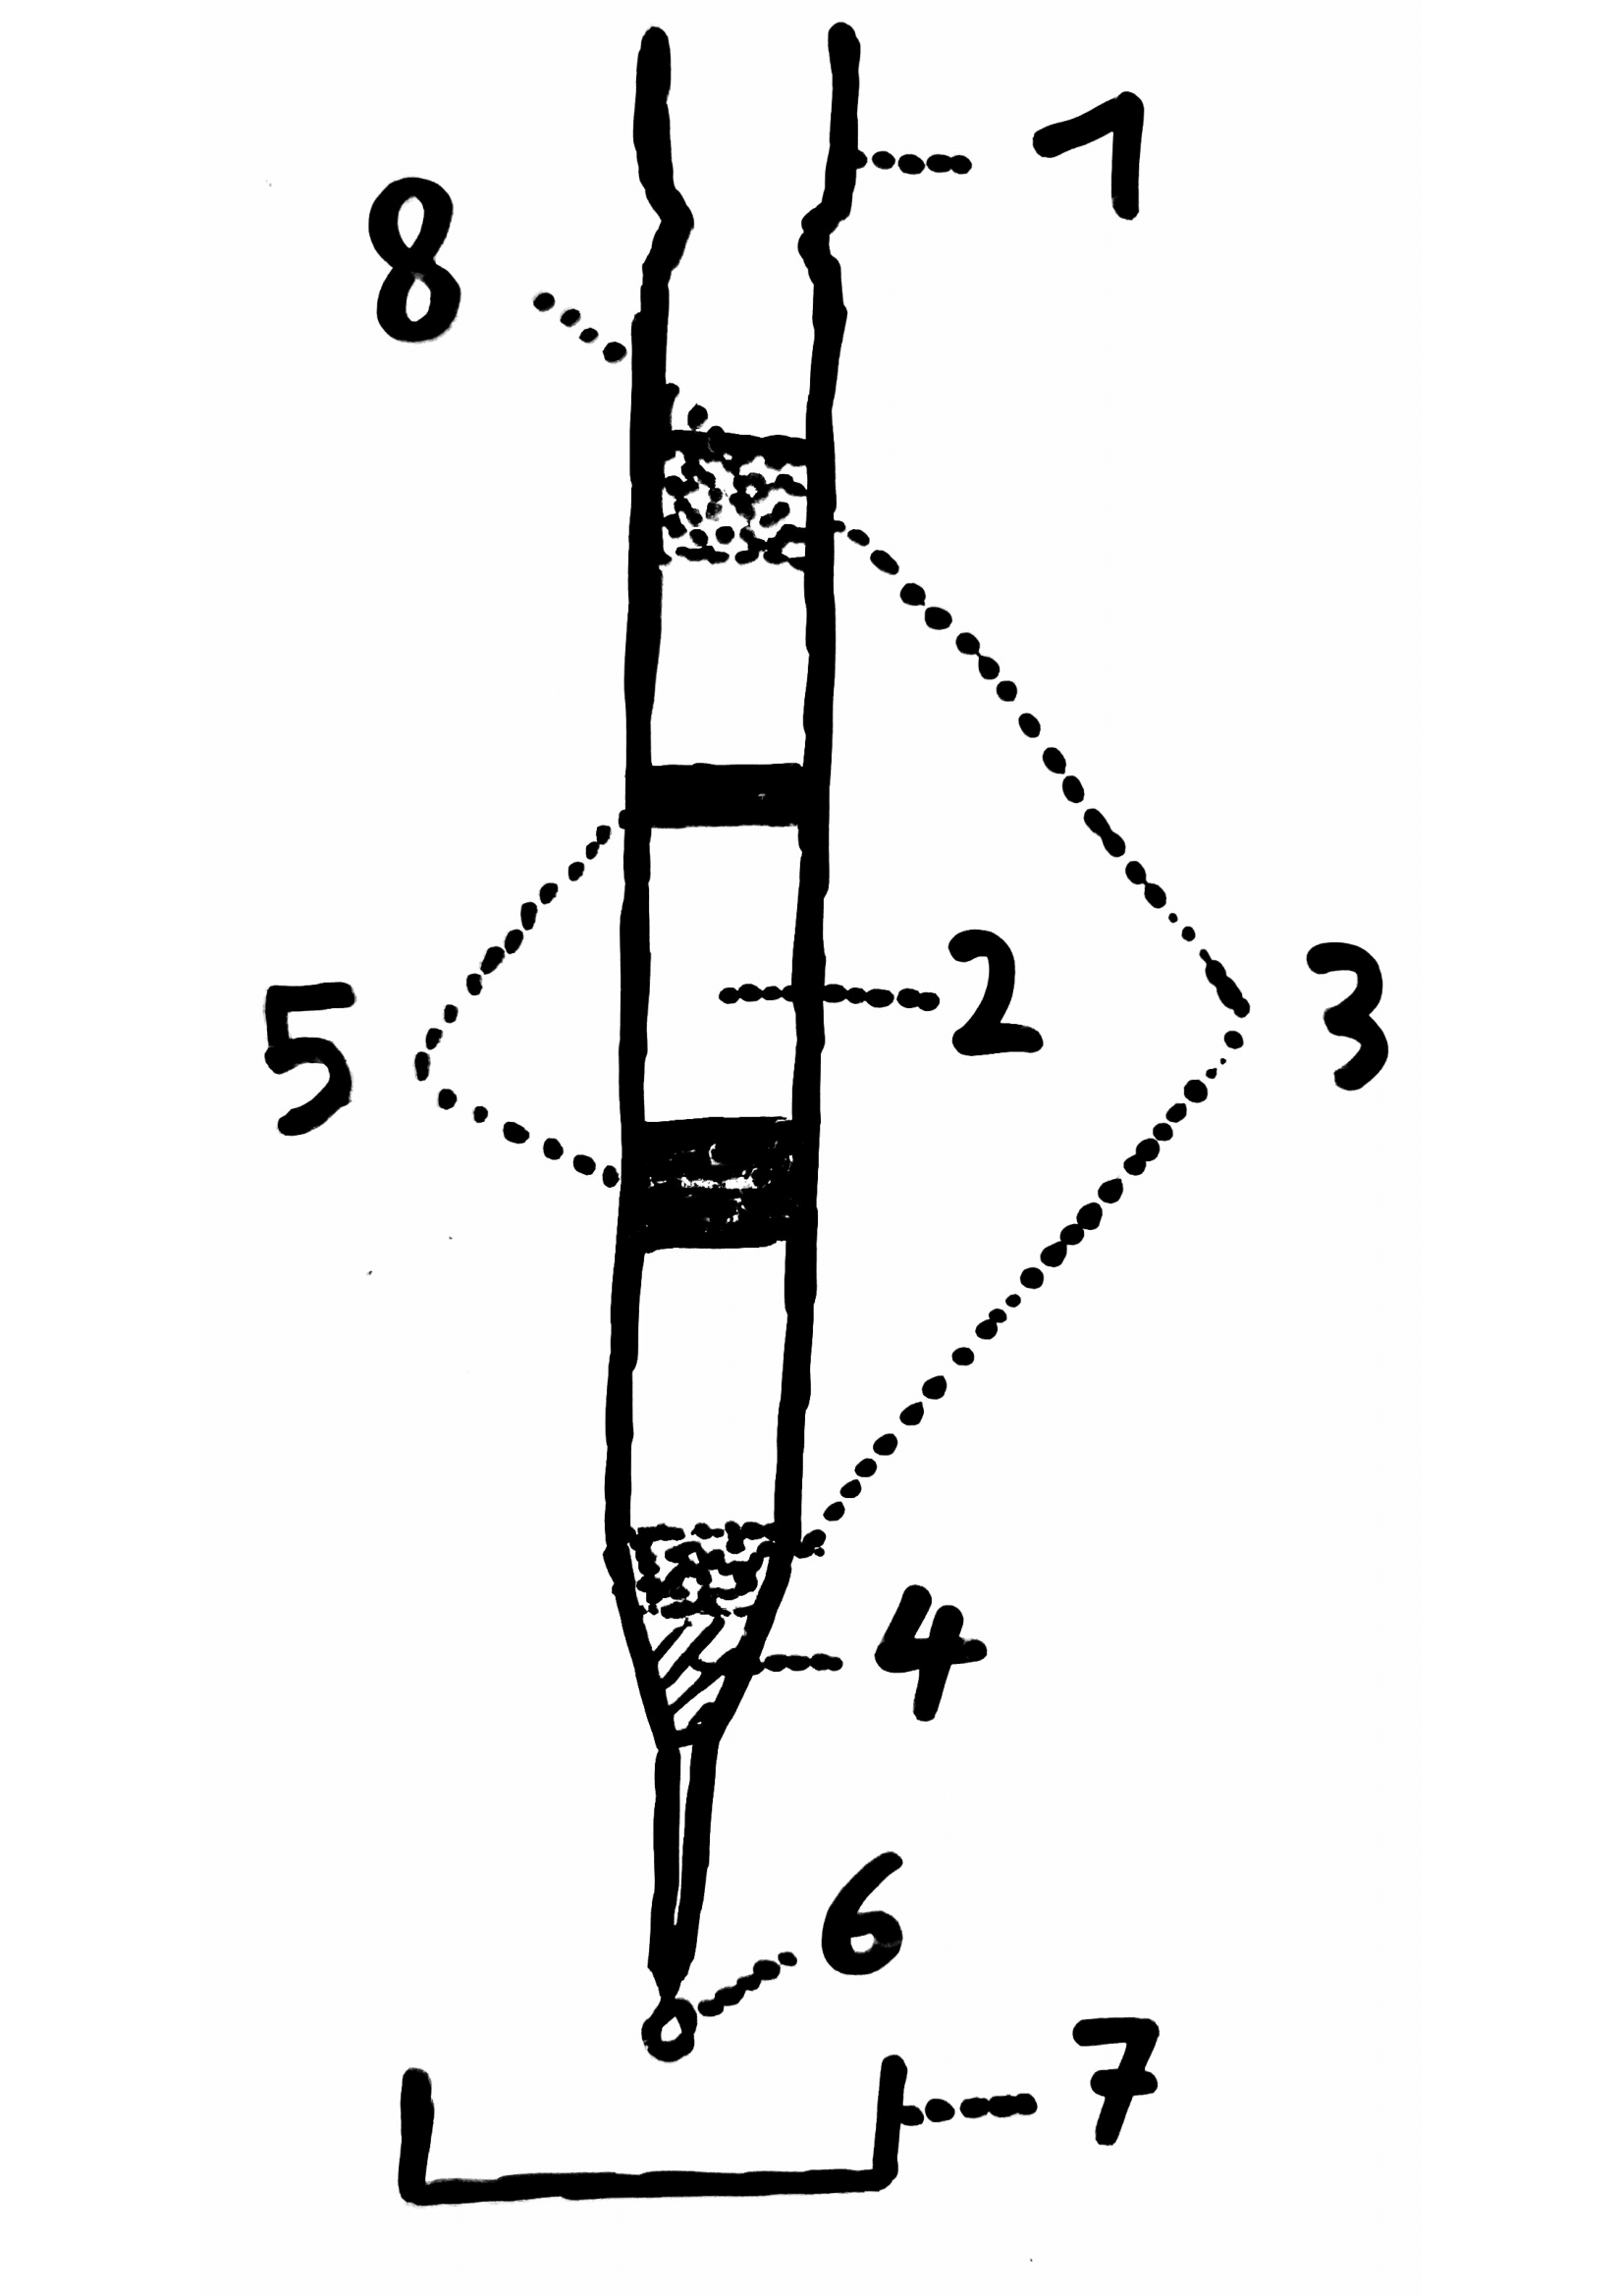
\includegraphics[scale=0.08, center]{Graphiken/Versuchsanordnungen/VersuchsanordnungSC.png} 
          \caption[schematische Versuchsanordnung Säulenchromatographie, Quelle: Autor]{schematische Versuchsanordnung: (1) Pasteurpipette - Säule - und Öffnung für Eluentenzufuhr, (2) \ch{Al2O3}-Schicht, (3) Sand, (4) Glaswolle bzw. Watte, (5) Banden der getrennten Substanzen, (6) Ort der Elution der Substanz, (7) Auffangvorrichtung, (8) Aufgabe der Probe}
          \label{fig:Versuchsanordnungzwei}
        \end{figure}
        
        Im ersten Schritt wurde eine Analysenlösung vorbereitet. Dazu wurde ein Spinatblatt im \SI[mode=text,separate-uncertainty=true]{50}{\milli\litre} Becherglas zerkleinert und mit ca. \SI[mode=text]{5}{\milli\litre} \ch{EtOH} gewaschen. Die \ch{EtOH}-Fraktion wurde abdekantiert und verworfen. Nun wurden \SI[mode=text]{5}{\milli\litre} Petrolether hinzugegeben und das Blattextrakt für ca. \SI[mode=text]{5}{\minute} lang durch Schütteln extrahiert. Die Petrolether-Fraktion wurde in ein Sammelgefäß abdekantiert und nicht zur Trennung eingesetzt. 
        
        Nun wurden die Elutionslösungen\footnote{=mobilen Phase} vorbereitet. Elutionslösung 1 war eine Mischung von \SI[mode=text]{0.7}{\milli\litre} Aceton mit \SI[mode=text]{9.3}{\milli\litre} Petrolether\footnote{im Messzylinder abgemessen}. Elutionslösung 2 war reines Aceton. Beide Lösungen wurden griffbereit aufbewahrt.
        
        Die Trennsäule wurde wie in \ref{fig:Versuchsanordnungzwei} skizziert vorbereitet. Als Säule diente eine Pasteurpipette, die man mit einer Klammer an einem Stativ befestigte. Zuerst wurde die Pipette mit Watte befüllt, die mithilfe einer zweiten Pasteurpipette schön kompakt zusammengedrückt wurde. Danach wurde diese mit einer ca. \SI[mode=text]{0.4}{\centi\meter} hohen Sandschicht überdeckt. In einem Reagenzglas wurde eine ca. \SI[mode=text]{1}{\centi\meter} dicke \ch{Al2O3}-Schicht mit \SI[mode=text]{7}{\centi\meter} Petrolether überdeckt. Durch Aufschlemmen des \ch{Al2O3} mit einer Pasteurpipette  erhielt man eine Suspension, die in die Säule überführt wurde, wobei darauf geachtet wurde, die Entstehung von Luftblasen in der Säule zu vermeiden. Die \ch{Al2O3}-Schicht stand etwa \SI[mode=text]{6}{\centi\meter} hoch. Ein Trockenlaufen der Säule wurde in allen folgenden Schritten durch konstante Zufuhr an Petrolether bzw. später Elutionslösung verhindert\footnote{beim Befüllen nach dem Trockenlaufen kann es zum Einschluss von Luft in der Säule kommen, was die Trennleistung reduziert}. Diese Schicht wurde mit einer ca. \SI[mode=text]{0.5}{\centi\meter} hohen Sandschicht überdeckt. 
        
        Nun konnte mit der Trennung gestartet werden. Dazu wurde eine vom Praktikumsleiter vorgelegte Analysenlösung auf die oberste Sandschicht gelegt\footnote{nachdem der Petrolether gerade die oberste Sandschicht durchquert hatte} und gewartet, bis sie zur Gänze in die Sandschicht eingedrugen war\footnote{Vorgang auch als Beladen der Säule bezeichnet}. Elutionslösung 1 wurde hinzugegeben. Das Carotin löste sich in dieser besser wie das Chlorophyll und eine gelbe Bande wanderte die Säule hinunter. Am Säulenende angelangt, wurde die Fraktion in einem Zentrifugenröhrchen aufgefangen, wie in \ref{fig:Versuchsanordnungzwei} gezeigt. Das Chlorophyll wurde durch einen Wechsel der Elutionslösung erhalten. Dazu wurde Elutionslösung 2 verwendet. Analog zum Carotin wurde das Chlorophyll am Säulenende aufgefangen.
        
    \subsection{Ergebnisse und Diskussion}
    
      Nach dem Trennvorgang wurden zwei Lösungen erhalten - eine mit Carotin und eine weitere mit Chlorophyll. Durch die unterschiedliche Farbe können sie eindeutig voneinander unterschieden werden. Die hohe Farbintensität der beiden Lösungen deutet auf eine effiziente Trennung hin, was durch die recht scharfe Bande der Carotin-Lösung bestätigt wird - siehe Abbildungen \ref{fig:LosungenCarotin} und \ref{fig:TrennungCarotin}. Lufteinschlüsse wurden nicht beobachtet und es kam während der Trennung zu keinem Trockenlaufen der Säule. Die Trennung wird somit als erfolgreich angesehen.
      
      \begin{figure}[H]
        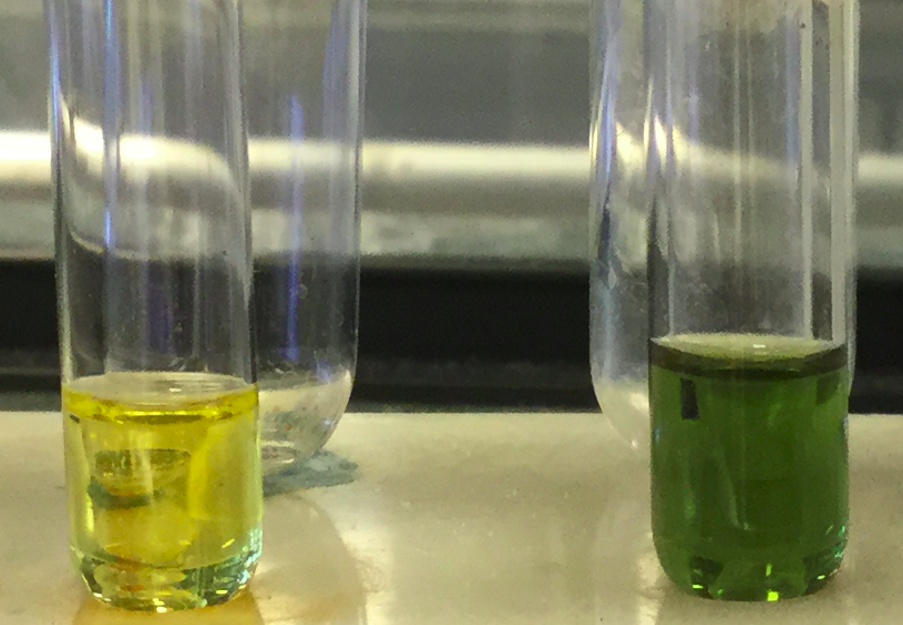
\includegraphics[scale=0.25, center]{Graphiken/Versuchsanordnungen/LosungenSubstanzen.png} 
        \caption[gesammelten Eluenten der Säulenchromatographie, Quelle: Autor]{(links) Carotin-Lösung, (rechts) Chlorophyll-Lösung}
        \label{fig:LosungenCarotin}
      \end{figure}
      
      Nach der Zugabe von Aceton wurde beobachtet, dass neben der grünen Chlorophyll-Bande, die kontinuierlich nach unten wanderte eine zusätzliche grüne Bande vorhanden war, die sich jedoch am Anfang der Säule \textit{festsetzte} und offensichtlich nicht im Aceton löste - siehe Abbildung \ref{fig:TrennungChlorophyll}. Dies ist auf etwas feste, grüne Blattsubstanz zurückzuführen, die noch in der Probelösung vorhanden war. 
      
      \begin{figure}
        \centering
        \begin{subfigure}{.5\textwidth}
          \centering
          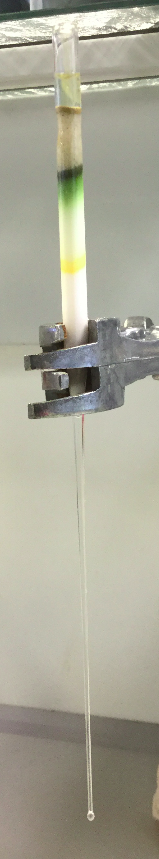
\includegraphics[width=.4\linewidth]{Graphiken/Versuchsanordnungen/SauleTrennungCarotinbande.png}
          \caption{Aufbau der Säule und Carotin-Bande}
          \label{fig:TrennungCarotin}
        \end{subfigure}%
        \begin{subfigure}{.5\textwidth}
          \centering
          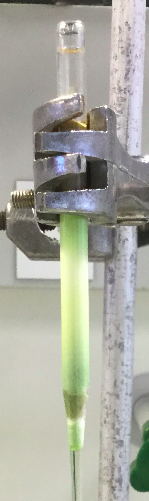
\includegraphics[width=.4\linewidth]{Graphiken/Versuchsanordnungen/TrennungChlorophyll.png}
          \caption{Chlorophyll-Bande kurz vor dem Auffangen}
          \label{fig:TrennungChlorophyll}
        \end{subfigure}
        \caption[Banden von Carotin und Chlorophyll, Quelle, Autor]{Banden von Carotin und Chlorophyll}
        \label{fig:TrennungSpinat}
      \end{figure}
      
  \pagebreak
  
  \printbibliography[title=Literaturverzeichnis]
  \listoffigures
  \listoftables
  
\end{document}
